\documentclass{wissdoc}
%\documentclass[oneside]{wissdoc}
% ----------------------------------------------------------------
% Bachelorarbeit - Hauptdokument
% ----------------------------------------------------------------
% wissdoc Optionen: draft, relaxed, pdf, oneside --> siehe wissdoc.cls
% ------------------------------------------------------------------
% Packages fuer Deckblatt
\usepackage[absolute]{textpos} 	%Textboxen an absolute Position setzen
\usepackage{setspace}						%Zeilenabstand anpassen
\usepackage{color}							%Farbige Schrift
\usepackage{graphicx}						%Einbinden von Grafiken

% Weitere packages: (Dokumentation dazu durch "latex <package>.dtx")
% \usepackage{varioref}
% \usepackage{verbatim}
% \usepackage{float}    %z.B. \floatstyle{ruled}\restylefloat{figure}
\usepackage{subfigure}
\usepackage[ngerman]{babel}
\usepackage[T1]{fontenc}
\usepackage[ansinew]{inputenc}

% Zeilenabstand nach Vorgabe - Falls gefordert
%\setstretch{1,3} 

% Inhaltsangabe auf Unterabschnitte(2 Ebenen) begrenzen
\setcounter{tocdepth}{2}


% \usepackage{color}    % Farbiger/grauer Text
% \usepackage{colortbl}   % Farbige/graue Tabellenzeilen und -spalten!! <--
% \usepackage{fancybox} % fuer schattierte,ovale Boxen etc.
% \usepackage{tabularx} % automatische Spaltenbreite
% \usepackage{supertab} % mehrseitige Tabellen
%% ---------------- end of usepackages -------------

%% Informationen fuer die PDF-Datei
\hypersetup{pdfauthor={Christian Fischer},%
            pdftitle={Bachelorarbeit},%
            pdfsubject={Konzeption und Implementierung einer Client-Server Anwendung fuer Gruppen- und Individualtransporte basierend auf Xamarin und .NET.},%
            pdfkeywords={Forschung, Entwicklung, Funktechnik},%
            pdfproducer={LaTeX},%
            pdfcreator={pdfLaTeX}
}

% Macros, nicht unbedingt notwendig
%%%%%%%%%%%%%%%%%%%%%%%%%%%%%%%%%%%%%%%%%%%%%%%%%%%%%%%%%%%
% macros.tex -- einige mehr oder weniger nuetzliche Makros
%%%%%%%%%%%%%%%%%%%%%%%%%%%%%%%%%%%%%%%%%%%%%%%%%%%%%%%%%%


%%%%%%%%%%%%%%%%%%%%%%%
% Kommentare 
%%%%%%%%%%%%%%%%%%%%%%%
\ifnotdraftelse{
\newcommand{\Kommentar}[1]{}
}{\newcommand{\Kommentar}[1]{{\em #1}}}
% Alles innerhalb von \Hide{} oder \ignore{} 
% wird von LaTeX komplett ignoriert (wie ein Kommentar)
\newcommand{\Hide}[1]{}
\let\ignore\Hide

%%%%%%%%%%%%%%%%%%%%%%%%%
% Leere Seite ohne Seitennummer, wird aber gezaehlt
%%%%%%%%%%%%%%%%%%%%%%%%%

\newcommand{\leereseite}{% Leerseite ohne Seitennummer, n�chste Seite rechts (wenn 2-seitig)
 \clearpage{\pagestyle{empty}\cleardoublepage}
}

%%%%%%%%%%%%%%%%%%%%%%%%%%
% Neue Seite rechts, leere linke Seite ohne Headings
%%%%%%%%%%%%%%%%%%%%%%%%%%
\newcommand{\xcleardoublepage}
{{\pagestyle{empty}\cleardoublepage}}

%%%%%%%%%%%%%%%%%%%%%%%%%%
% Tabellenspaltentypen (benoetigt colortbl)
%%%%%%%%%%%%%%%%%%%%%%%%%%
\newcommand{\PBS}[1]{\let\temp=\\#1\let\\=\temp}
\newcolumntype{y}{>{\PBS{\raggedright\hspace{0pt}}}p{1.35cm}}
\newcolumntype{z}{>{\PBS{\raggedright\hspace{0pt}}}p{2.5cm}}
\newcolumntype{q}{>{\PBS{\raggedright\hspace{0pt}}}p{6.5cm}}
\newcolumntype{g}{>{\columncolor[gray]{0.8}}c} % Grau
\newcolumntype{G}{>{\columncolor[gray]{0.9}}c} % helleres Grau

%%%%%%%%%%%%%%%%%%%%%%%%%%
% Anf�hrungszeichen oben und unten
%%%%%%%%%%%%%%%%%%%%%%%%%%
\newcommand{\anf}[1]{"`{#1}"'}

%%%%%%%%%%%%%%%%%%%%%%%%%%
% Tiefstellen von Text
%%%%%%%%%%%%%%%%%%%%%%%%%%
% S\tl{0} setzt die 0 unter das S (ohne Mathemodus!)
% zum Hochstellen gibt es uebrigens \textsuperscript
\makeatletter
\DeclareRobustCommand*\textlowerscript[1]{%
  \@textlowerscript{\selectfont#1}}
\def\@textlowerscript#1{%
  {\m@th\ensuremath{_{\mbox{\fontsize\sf@size\z@#1}}}}}
\let\tl\textlowerscript
\let\ts\textsuperscript
\makeatother

%%%%%%%%%%%%%%%%%%%%%%%%%%
% Gau�-Klammern
%%%%%%%%%%%%%%%%%%%%%%%%%%
\newcommand{\ceil}[1]{\lceil{#1}\rceil}
\newcommand{\floor}[1]{\lfloor{#1}\rfloor}

%%%%%%%%%%%%%%%%%%%%%%%%%%
% Average Operator (analog zu min, max)
%%%%%%%%%%%%%%%%%%%%%%%%%%
\def\avg{\mathop{\mathgroup\symoperators avg}}

%%%%%%%%%%%%%%%%%%%%%%%%%%
% Wortabk�rzungen
%%%%%%%%%%%%%%%%%%%%%%%%%%
\def\zB{z.\,B.\ }
\def\dh{d.\,h.\ }
\def\ua{u.\,a.\ }
\def\su{s.\,u.\ }
\newcommand{\bzw}{bzw.\ }

%%%%%%%%%%%%%%%%%%%%%%%%%%%%%%%%%%%
% Einbinden von Graphiken
%%%%%%%%%%%%%%%%%%%%%%%%%%%%%%%%%%%
% global scaling factor
\def\gsf{0.9}
%% Graphik, 
%% 3 Argumente: Datei, Label, Unterschrift
\newcommand{\Abbildung}[3]{%
\begin{figure}[tbh] %
\centerline{\scalebox{\gsf}{\includegraphics*{#1}}} %
\caption{#3} %
\label{#2} %
\end{figure} %
}
\let\Abb\Abbildung
%% Abbps
%% Graphik, skaliert, Angabe der Position
%% 5 Argumente: Position, Breite (0 bis 1.0), Datei, Label, Unterschrift
\newcommand{\Abbildungps}[5]{%
\begin{figure}[#1]%
\begin{center}
\scalebox{\gsf}{\includegraphics*[width=#2\textwidth]{#3}}%
\caption{#5}%
\label{#4}%
\end{center}
\end{figure}%
}
\let\Abbps\Abbildungps
%% Graphik, Angabe der Position, frei w�hlbares Argument f�r includegraphics
%% 5 Argumente: Position, Optionen, Datei, Label, Unterschrift
\newcommand{\Abbildungpf}[5]{%
\begin{figure}[#1]%
\begin{center}
\scalebox{\gsf}{\includegraphics*[#2]{#3}}%
\caption{#5}%
\label{#4}%
\end{center}
\end{figure}%
}
\let\Abbpf\Abbildungpf

%%
% Anmerkung: \resizebox{x}{y}{box} skaliert die box auf Breite x und H�he y,
%            ist x oder y ein !, dann wird das uspr�ngliche 
%            Seitenverh�ltnis beibehalten.
%            \rescalebox funktioniert �hnlich, nur das dort ein Faktor
%            statt einer Dimension angegeben wird.
%%
% \Abbps{Position}{Breite in Bruchteilen der Textbreite}{Dateiname}{Label}{Bildunterschrift}
%

\newcommand{\refAbb}[1]{%
s.~Abbildung \ref{#1}}

%%%%%%%%%%%%%%%%%%%%
%% end of macros.tex
%%%%%%%%%%%%%%%%%%%%

% Print URLs not in Typewriter Font
\def\UrlFont{\rm}

%\newcommand{\blankpage}{% Leerseite ohne Seitennummer, naechste Seite rechts
% \clearpage{\pagestyle{empty}\cleardoublepage}
%}

%% Einstellungen fuer das gesamte Dokument

% Trennhilfen
% Wichtig!
% Im german-paket sind zusaetzlich folgende Trennhinweise enthalten:
% "- = zusaetzliche Trennstelle
% "| = Vermeidung von Ligaturen und moegliche Trennung (bsp: Schaf"|fell)
% "~ = Bindestrich an dem keine Trennung erlaubt ist (bsp: bergauf und "~ab)
% "= = Bindestrich bei dem Worte vor und dahinter getrennt werden duerfen
% "" = Trennstelle ohne Erzeugung eines Trennstrichs (bsp: und/""oder)

% Trennhinweise fuer Woerter hier beschreiben
\hyphenation{
% Pro-to-koll-in-stan-zen
% Ma-na-ge-ment  Netz-werk-ele-men-ten
% Netz-werk Netz-werk-re-ser-vie-rung
% Netz-werk-adap-ter Fein-ju-stier-ung
% Da-ten-strom-spe-zi-fi-ka-tion Pa-ket-rumpf
% Kon-troll-in-stanz
}

%Tabellen Kommandos
\newcolumntype{L}[1]{>{\raggedright\arraybackslash}p{#1}}
\newcolumntype{C}[1]{>{\centering\arraybackslash}p{#1}}
\newcolumntype{R}[1]{>{\raggedleft\arraybackslash}p{#1}}

% Index-Datei oeffnen
\ifnotdraft{\makeindex}
%%%%%%%%%%%%%% includeonly %%%%%%%%%%%%%%%%%%%
% Es werden nur die Teile eingebunden, die hier aufgefuehrt sind!
%\includeonly{%
%titelseite,%
%erklaerung,%
%kurzfassung,%
%einleitung,%
%analyse,%
%entwurf,%
%implemen,%
%zusammenf%
%}
%%%%%%%%%%%%%%%%%%%%%%%%%%%%%%%%%%%%%%%%%%%%%%
\begin{document}
%Auskommentiert, da nicht notwendig fuer das Praktikum
%\ifnotdraft{
	%%%%Vorlage
	\begin{figure}[t]
			\hspace{-2.2cm}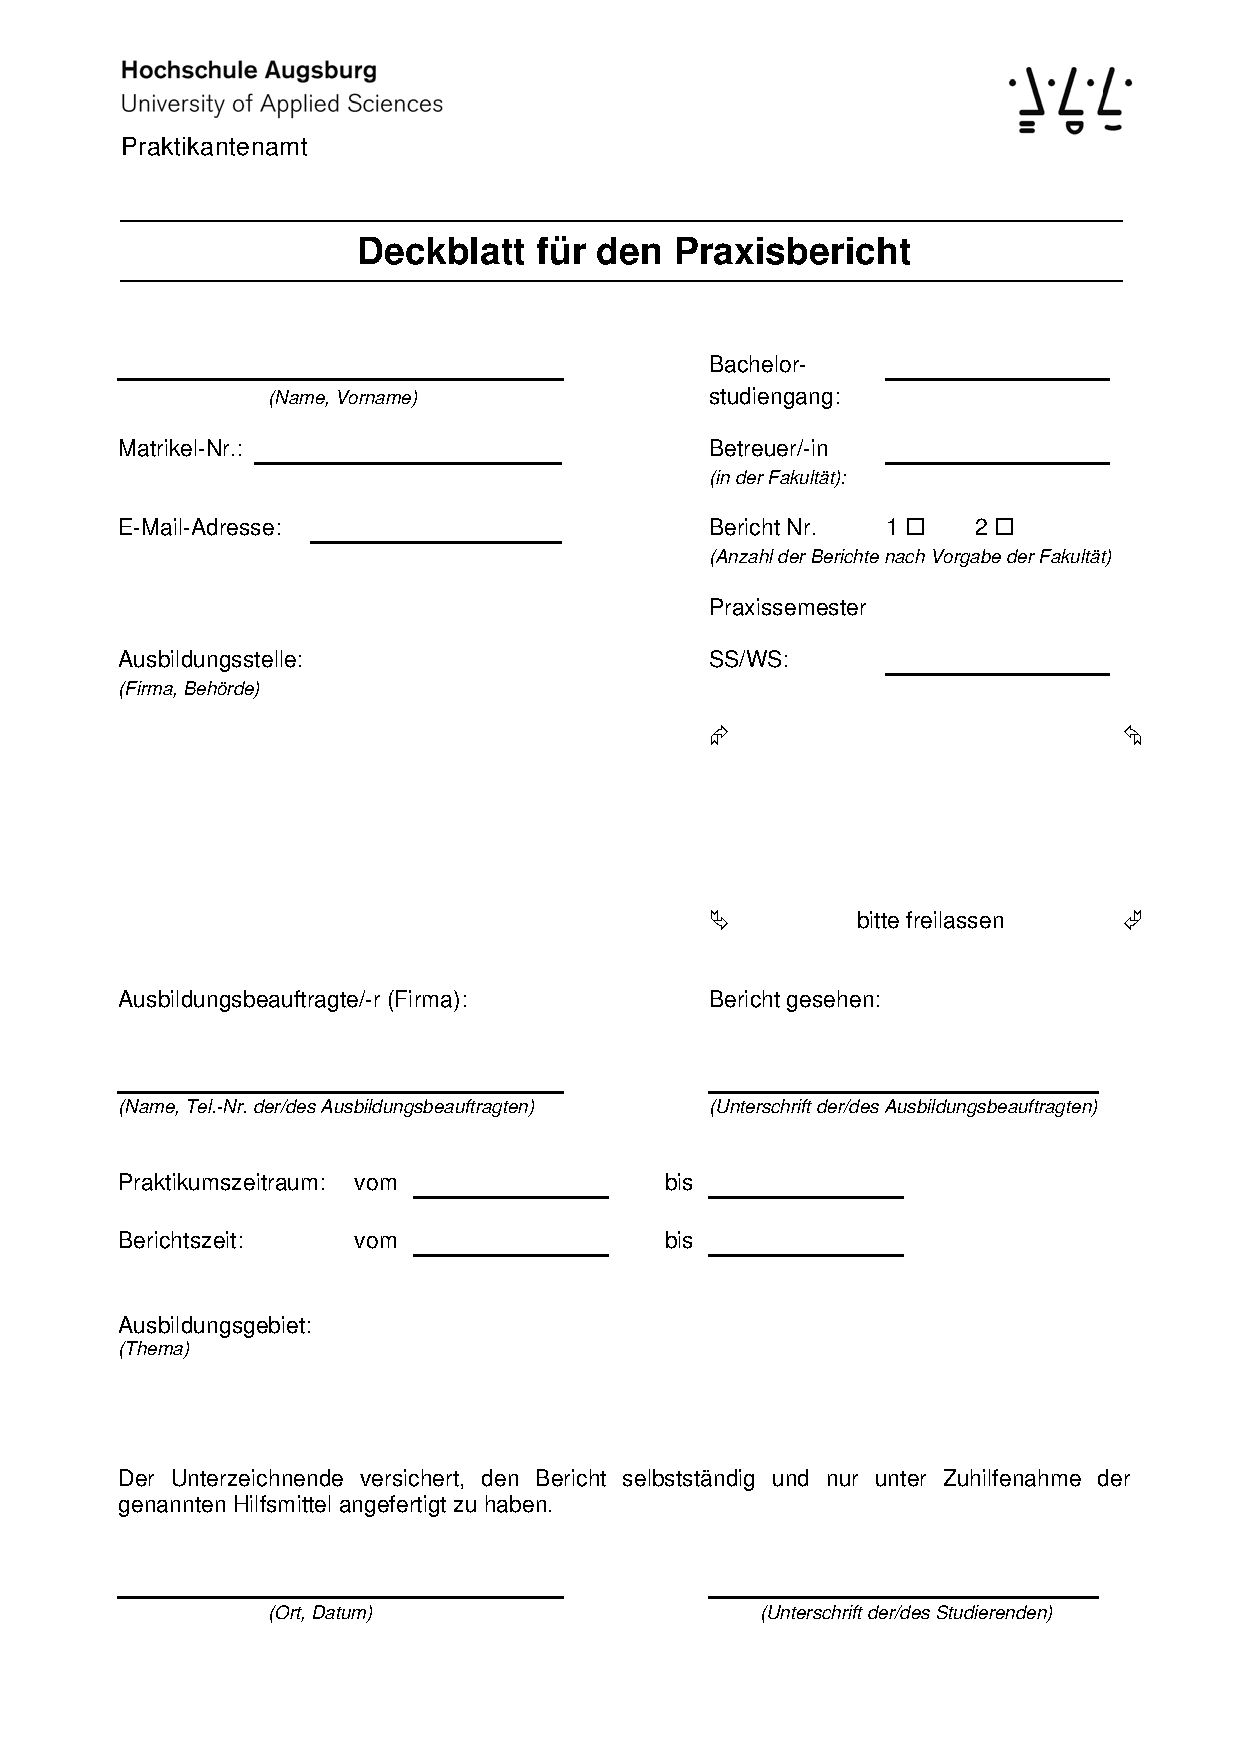
\includegraphics[width=0.93\paperwidth]{figures/deckblatt_prax_bac}
		\label{fig:deckblatt_prax_bac}
	\end{figure}  %<-- Nach Vorgabe der HS Augsburg

	\textblockorigin{20mm}{30mm}

\thispagestyle{empty}\null
%%%%Logo - Hochschule Augsburg - Informatik
\begin{textblock}{10}(8.0,1.1)
\begin{figure}[h]
	\centering
		
\includegraphics[width=0.45\textwidth]{logos/hsa_informatik_logo_lq.pdf}
\end{figure}

\end{textblock}

%%% Text unter Logo
\begin{textblock}{15}(12.43,2.1)
	\LARGE
	\textsf{
		\textbf{\textcolor[rgb]{1,0.41,0.13}{\\
			\begin{flushleft}
				Fakultaet fuer\\
				Informatik\\
			\end{flushleft}
			}
		}
	}
\end{textblock}

%%%%Textbox links - Informationen
\begin{textblock}{15}(2,1.4)
	%\LARGE
	\begin{flushleft}
		\begin{spacing} {1.2}
			\huge	
				\textcolor[rgb]{1,0.41,0.13}{\\
				\textbf{Bachelorarbeit}}\\
				\vspace{60pt}
			\LARGE
				Studienrichtung\\
				Informatik\\
				\vspace{40pt}
				
				Christian Fischer\\
				\vspace{30pt}		
				Matrikelnummer: 945609\\
				\vspace{30pt}
				Thema: Konzeption und Implementierung einer Client-Server Anwendung\\ f\"ur Gruppen- und Individualtransporte basierend auf Xamarin und .NET.\\
				\vspace{60pt}		
			\LARGE
				Pr\"ufer: \\
				\vspace{10pt}		
				Abgabedatum: \\
			\end{spacing}
		\end{flushleft}
		
\end{textblock}



%%%%Textbox rechts - Hochschule
\begin{textblock}{5}(12.45,9.0)
	\scriptsize
	\textcolor[rgb]{1,0,0}{\\
		\begin{flushleft}
			\begin{spacing} {1.3}
				Hochschule fuer angewandte\\
				Wissenschaften Augsburg\\
				\vspace{4pt}
				An der Hochschule 1\\
				D-86161 Augsburg\\
				\vspace{4pt}
				Telefon +49 821 55 86-0\\
				Fax +49 821 55 86-3222\\
				www.hs-augsburg.de\\
				info(at)hs-augsburg-de
			\end{spacing}
		\end{flushleft}
		}
\end{textblock}


%%%%Textbox rechts unten - Fakultaet und Autor
\begin{textblock}{5}(12.45,11.5)
	\scriptsize
		\begin{flushleft}
			\begin{spacing} {1.3}
				Fakultaet fuer Informatik\\
				Telefon +49 821 55 86-3450\\
				Fax \hspace{10pt} +49 821 55 86-3499\\
				\vspace{6pt}
				Verfasser der Bachelorarbeit\\
				Christian Fischer\\
				Josef-Priller-Strasse 40\\
				86159 Augsburg\\
				Telefon +49 157/7280891\\
				stchfisc@hs-augsburg.de\\
			\end{spacing}
		\end{flushleft}
	\end{textblock}
\pagebreak  %<-- Nach Vorgabe der HS Augsburg
	%
	%%%% Innere Titelseite 
 	%\include{titelseite} %<-- Vorgabe Pruefer oder frei waehlbar
	%
	%%%%Optional - Falls von der Firma gefordert
	%\include{sperrvermerk}
	%
	%%%%Pflicht
 	%\include{erklaerung}
	%
	%%% Leere Seite bei zweiseitigem Druck
	%\ifnotonesideelse{\blankpage}{}
	%\include{kurzfassung}
	%%% Leere Seite bei zweiseitigem Druck
	%\ifnotonesideelse{\blankpage}{}
%}



%
%% ++++++++++++++++++++++++++++++++++++++++++
%% Verzeichnisse
%% ++++++++++++++++++++++++++++++++++++++++++
\pagenumbering{roman}
\ifnotdraft{
\tableofcontents
% Leere Seite bei zweiseitigem Druck
%\ifnotonesideelse{\blankpage}{}
%\listoffigures
%% Leere Seite bei zweiseitigem Druck
%\ifnotonesideelse{\blankpage}{}
%\listoftables
%% Leere Seite bei zweiseitigem Druck
%\ifnotonesideelse{\blankpage}{}
}
%% ++++++++++++++++++++++++++++++++++++++++++
%% Hauptteil
%% ++++++++++++++++++++++++++++++++++++++++++
\graphicspath{{figures/}}
\pagenumbering{arabic}

%%% Ab hier eigene Kapitel einfuegen
%%% Kapitel sind analog zur Wordvorlage zu waehlen

                                               
\chapter{Einleitung}


\section{Thema Beschreibung}
Text kommt

\section{Motivation}
Text kommt

\section{Projektziele und/oder Aufgabenbereiche}
Text kommt

\section{Inhaltsangabe}
Text kommt


\chapter{Stand der Technik}

\chapter{Analyse}

\section{Datensammlung}
Text kommt

\section{Auswertung}
Text kommt

\section{Ergebnisse}
Text kommt


\chapter{Planung}

\section{Userstories}
Text kommt

\section{Entwurf}
Text kommt

\subsection{Personas}

Text kommt
\subsection{MockUps}
Text kommt


\chapter{Implementierung}

\section{Projektbeschreibung}
Text kommt

\section{Arbeitsschritte/Arbeitsablauf}
Text kommt

\subsection{Eigene Arbeitspakete/Taetigkeiten}
Text kommt


\chapter{Ausblick}



\chapter{Zusammenfassung}



\chapter{Beispiel - Kapitel}
\label{ch:Beispiele}
%% ==============================
Beispiele\ldots



\section{Zitieren}
Quellen\cite{li00,jackson91,lakhina04a,netflow,rfc2386} 
nicht vergessen. Dazu verwendet ihr bibtex.

%% ==============================
\section{Bild einfuegen}
%% ==============================

\subsection{Ein Bild skaliert}

\begin{figure}[htbp]%Positionierung vorzugsweise an dieser Stelle. Falls nicht moeglich oben positionieren. Falls das auch nicht geht unten.
	\centering
		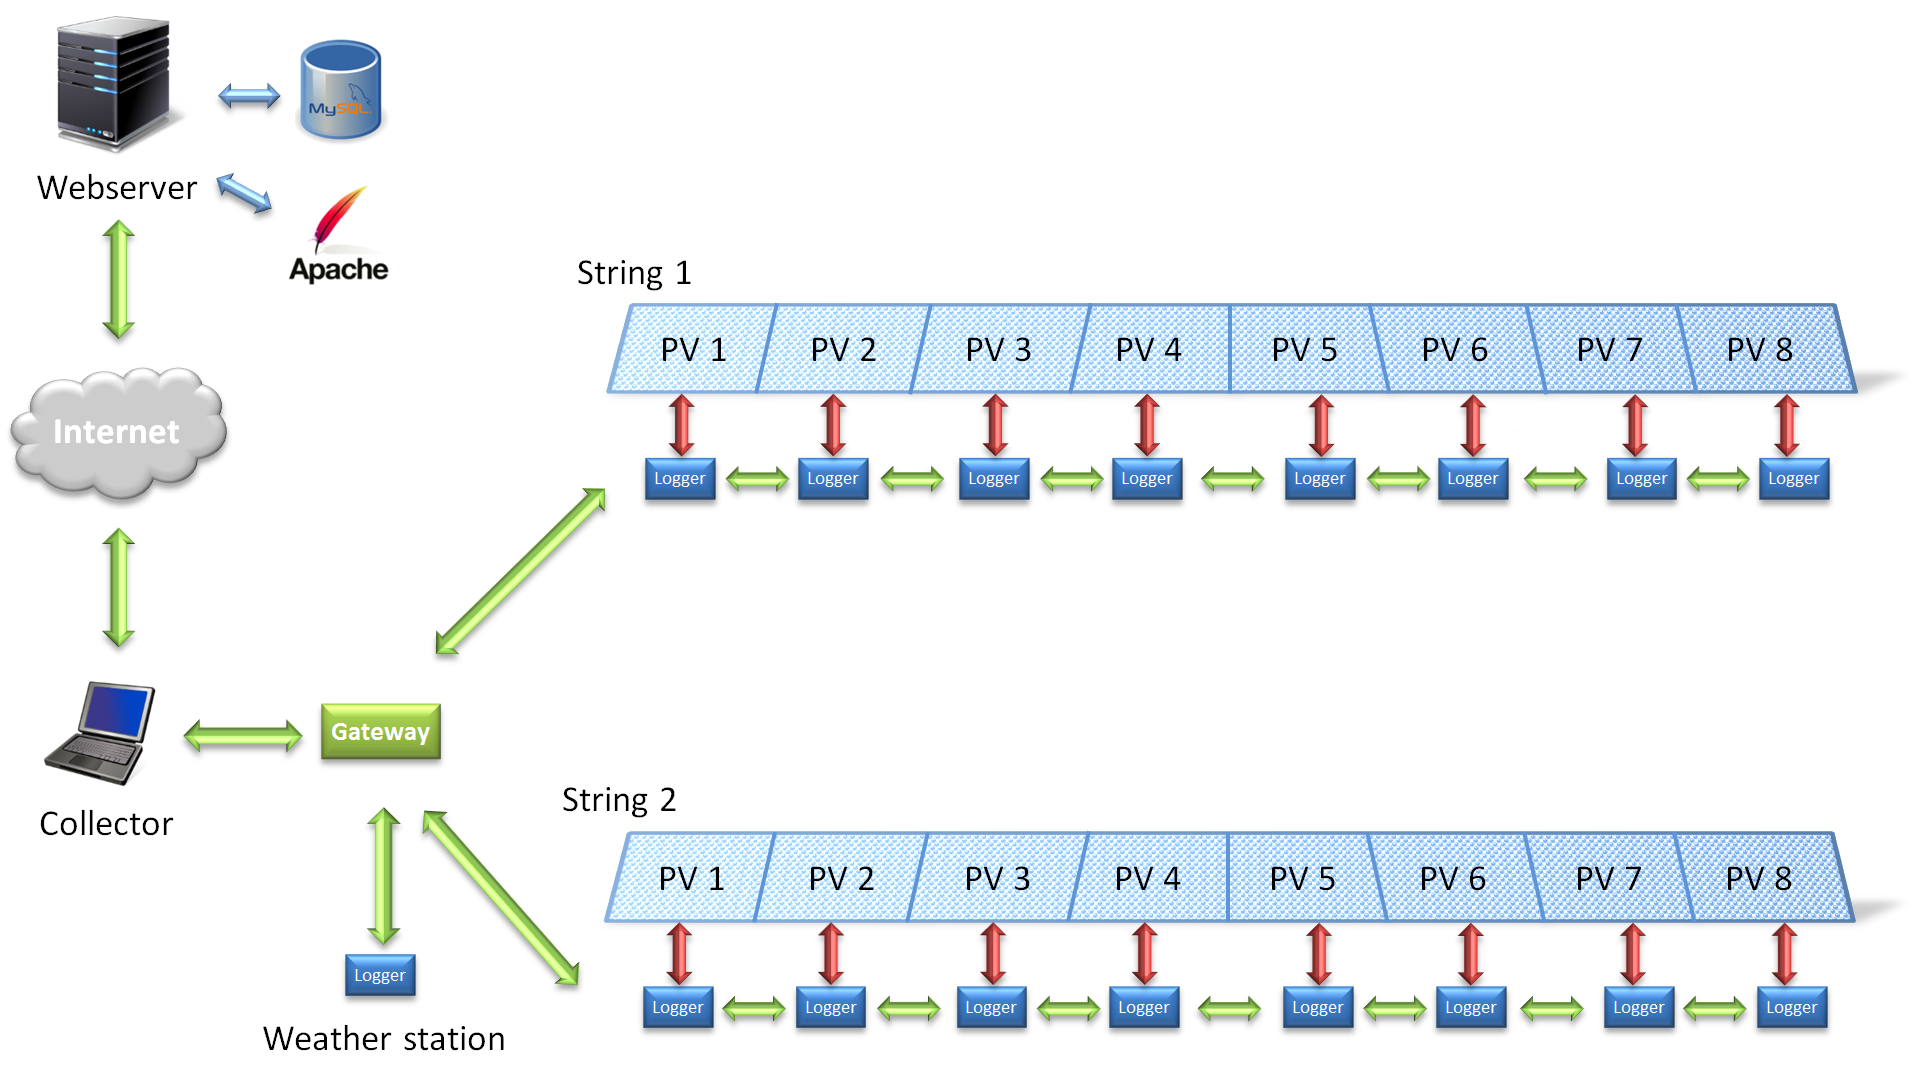
\includegraphics[width=0.80\textwidth]{../figures/large1.png}
	\caption{Beschriftungstext}
	\label{fig:large1}
\end{figure}

\subsection{Zwei Bilder nebeneinander oder untereinander}
%%%%%%%%%%%%%%%%%%%%%%%%%%%%%%%
\begin{figure*}[!htb]
	\centering
	\subfigure[Beschriftung Bild links]{
	  \label{fig:small1}
		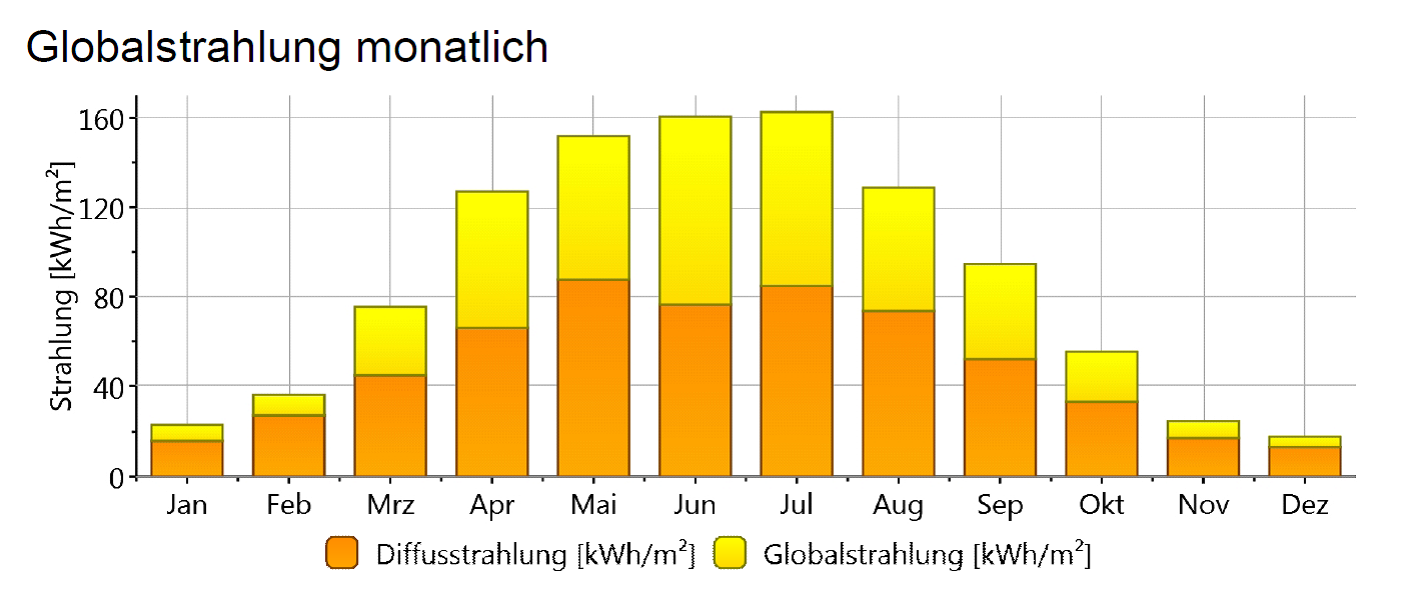
\includegraphics[angle=0,width=0.68\textwidth]{../figures/small1.png}}
	\subfigure[Beschriftung Bild rechts]{
	  \label{fig:small2}
		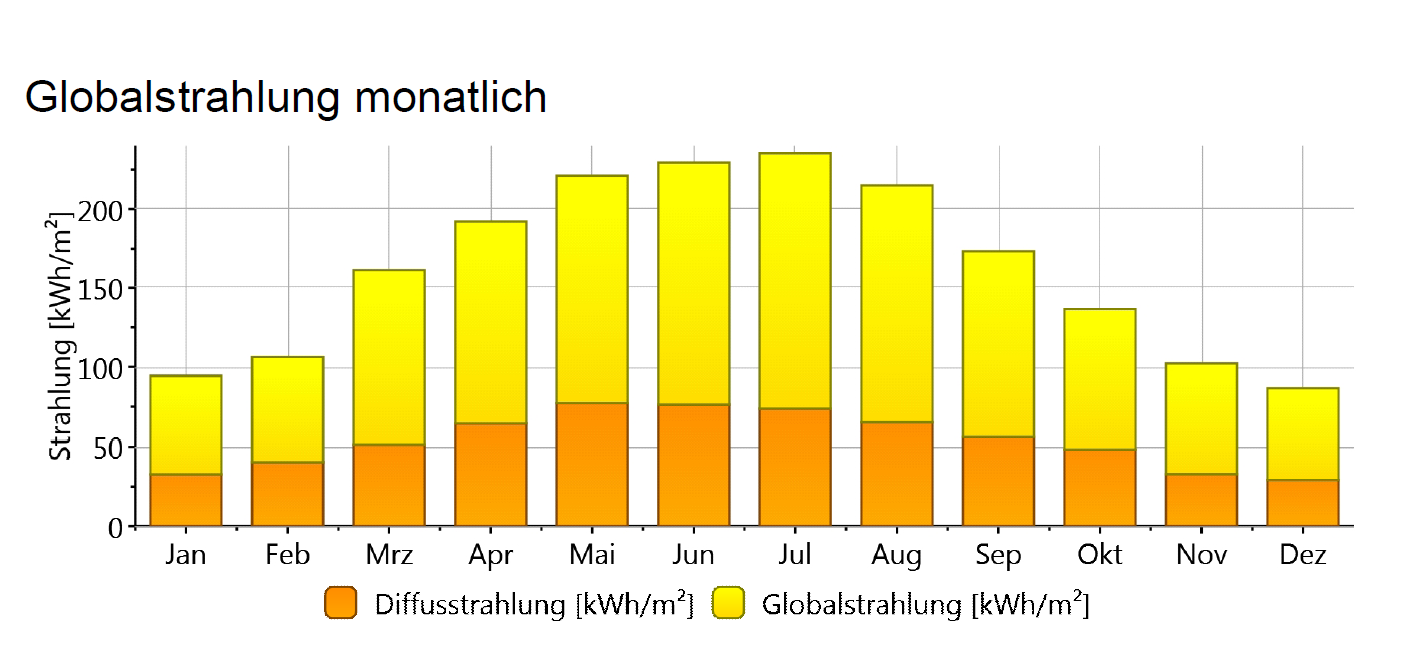
\includegraphics[angle=0,width=0.68\textwidth]{../figures/small2.png}}
 	\caption{Beschriftung beide Bilder} 
	\label{fig:beidebilder}
\end{figure*}
%%%%%%%%%%%%%%%%%%%%%%%%%%%%%%%


%% ==============================
\section{Tabellen}
%% ==============================
\begin{table}[htbp]
	\centering
		\begin{tabular}{|l|L{3.3 cm}|L{6.1 cm}|}
			\hline
			Firma								&			Produkte / Loesungen											&		WEB\\
			\hline
			Concentrix (Soitec)	&	Module mit Konzentratoren (Fresnel-Linsen)	&	http://www.soitec.com \\
			\hline
			Isofoton						&	Module mit Konzentratoren (Fresnel-Linsen)	&	http://www.isofoton.com \\
			\hline
			Semprius						& Module mit Konzentratoren (Fresnel-Linsen)	& http://www.semprius.com \\ 
			\hline
			\hline
			Azur Space					& Mehrfach Junction Zellenhersteller					& http://www.azurspace.com \\
			\hline
			Cyrium Technologies	& Mehrfach Junction Zellenhersteller					& \small{http://www.cyriumtechnologies.com} \\
			\hline
			Emcore							& Mehrfach Junction Zellenhersteller					& http://www.emcore.com \\
			\hline
		\end{tabular}
	\caption{Hersteller von CPV-Produkten}
	\label{tab:Hersteller}
\end{table}

\begin{table}[htb]
		\centering
		%\renewcommand{\arraystretch}{1.03}
		\caption{Single-hop Scenario - Traffic Pattern \label{t:traffic}}
			
		\begin{tabular}{l@{~}l@{\,\,}l@{\,\,}l} \hline \rule{-2pt}{12pt}
			Pattern& Parameter & Distribution & Range/Values  \rule{0pt}{12pt} \\ \hline \rule{-2pt}{12pt}  
      \textbf{Burst}      
      & Burst IAT         & uniform  & [9.9; 10.1] s\\ 
      & Packets per Burst & constant & 100\\
      & Packet IAT        & constant & 0.02 s\\
      & Packet Size       & constant & 1024 bit\\
      & \# Sources & -        & 2\\
			& Offset						& uniform  & [0; 1] s\\ 
      \hline      \hline\rule{-2pt}{12pt} 
      \textbf{Single}     & Packet IAT        & uniform  & [0.9; 1.1] s\\
      & Packet Size       & constant & 1024 bit\\
      & \# Sources & -        & [10;20;30;40;50;\\
      & & & 60;70;80;90;100]\\
			& Offset						& uniform  & [0; 1] s\\ 
      \hline
    \end{tabular}
\end{table}


%% ++++++++++++++++++++++++++++++++++++++++++
%% Anhang
%% ++++++++++++++++++++++++++++++++++++++++++

%\appendix
%\include{anhang_a}
%\include{anhang_b}

%\ifnotonesideelse{\cleardoublepage}{}

%% ++++++++++++++++++++++++++++++++++++++++++
%% Literatur
%% ++++++++++++++++++++++++++++++++++++++++++
\addcontentsline{toc}{chapter}{\bibname}
%  mit dem Befehl \nocite werden auch nicht zitierte Referenzen abgedruckt 
% (normalerweise nicht erwuenscht)
% \nocite{*}
\bibliographystyle{rialpha}
%Einbinden Bibtexdatei - Direkt aus JabRef generiert
%\bibliography{literatur}
%% ++++++++++++++++++++++++++++++++++++++++++
%% Index (optional)
%% ++++++++++++++++++++++++++++++++++++++++++
%\ifnotdraft{
%\addcontentsline{toc}{chapter}{Index}
%\printindex            % Index, Stichwortverzeichnis
%}
\end{document}
